\begin{figure}[htbp]
  \begin{tabular}{ccc}
    \begin{minipage}{0.33\hsize}
      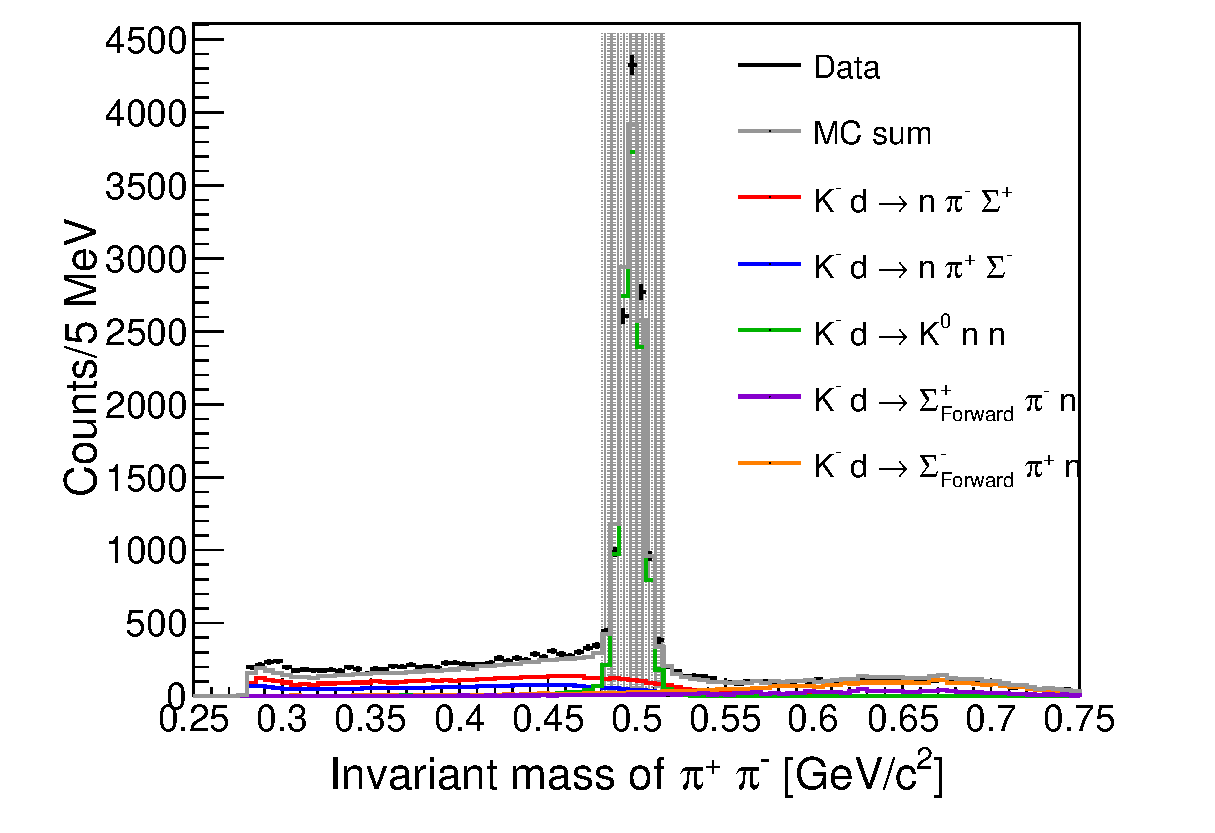
\includegraphics[width=4cm]{../pic/Dron/KN_ana/IM_pipi.eps}
    \end{minipage}
    \begin{minipage}{0.33\hsize}
      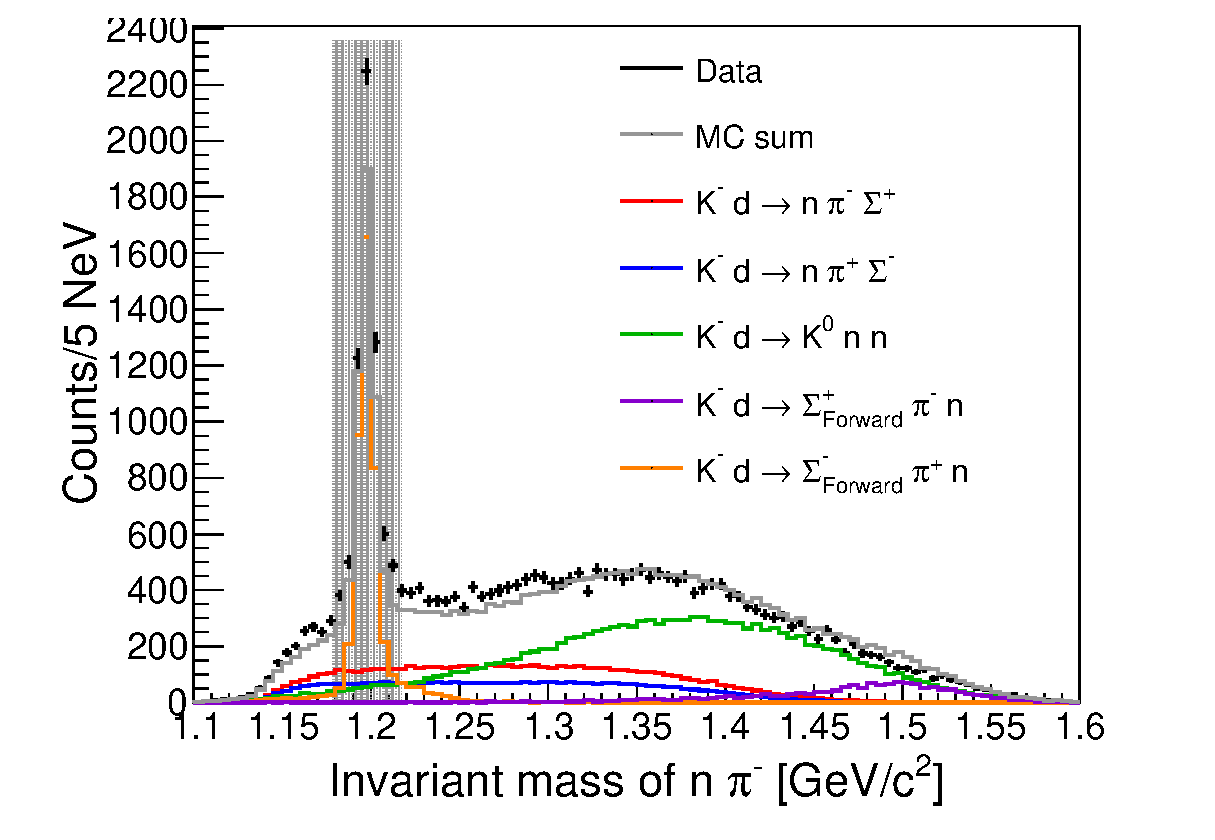
\includegraphics[width=4cm]{../pic/Dron/KN_ana/IM_npim.eps}
    \end{minipage}
    \begin{minipage}{0.33\hsize}
      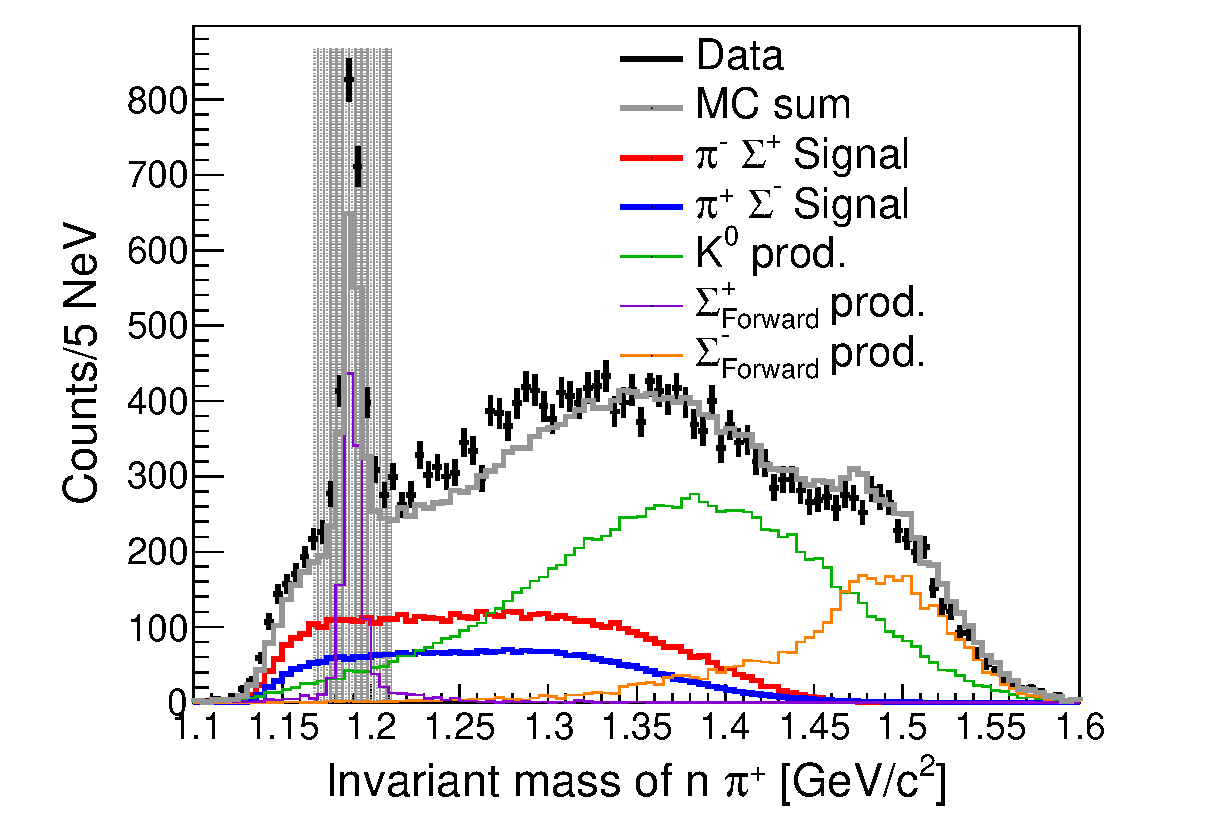
\includegraphics[width=4cm]{../pic/Dron/KN_ana/IM_npip.eps}
    \end{minipage}
  \end{tabular}

  \caption{
    The figures show template fitting for background estimation.
    The right, center, and left figures show invariant masses of $\pi^+ \pi^-$, $n \pi^-$ and $n \pi^+$, respectively.
    Error bars indicate data spectra.
    Bold lines indicate backward $\pi \Sigma$ production signals, red and blue indicate $\pi^- \Sigma^+$ and $\pi^+\Sigma^-$, respectively.
    The green, purple, and orange thin lines indicate the $K^0$, $\Sigma^-_{forward}$ and $\Sigma^+_{forward}$ production reactions.
    Gray lines indicate the sum of MC simulations.
    Gray hatching indicates the 3$\sigma$ rejection region estimated by fitting with Gaussian and polynomial backgrounds.
  }
  \label{fig:fit_IM}
\end{figure}
